\ifx\wholebook\relax \else

\documentclass[b5paper]{ctexart}
\usepackage[nomarginpar
  %, margin=.5in
]{geometry}

\addtolength{\oddsidemargin}{-0.05in}
\addtolength{\evensidemargin}{-0.05in}
\addtolength{\textwidth}{0.1in}
\usepackage[cn]{../../../prelude}

\setcounter{page}{1}

\begin{document}

\title{二叉堆}

\author{刘新宇
\thanks{{\bfseries 刘新宇 } \newline
  Email: liuxinyu95@gmail.com \newline}
  }

\maketitle
\fi

\markboth{二叉堆}{基本算法}

\ifx\wholebook\relax
\chapter{二叉堆}
\numberwithin{Exercise}{chapter}
\fi

\section{定义}
\label{introduction} \index{二叉堆}

堆是一种常见的数据结构,可以解决很多实际问题,包括排序、带有优先级的调度、实现图算法等\cite{wiki-heap}。堆有多种实现,最常见的一种通过数组来表示二叉树\cite{CLRS},进而实现堆。许多程序库中的堆都是这样实现堆的。由R.W. Floyd给出的高效堆排序算法也利用了这个实现\cite{wiki-heapsort}\cite{rosetta-heapsort}。堆本身的定义是抽象的,除数组外,它也可以由其它数据结构来实现。本章中,我们介绍那些由二叉树实现的堆,包括左偏堆(Leftist heap)、斜堆(Skew heap)、伸展堆(splay heap)\cite{okasaki-book}。一个堆或为空,或存有若干可比较大小的元素,并满足如下性质:

\begin{enumerate}
\item 堆顶总保存着最小(或最大)元素;
\item 弹出操作移除堆顶元素,并保持堆的性质1:新的堆顶元素仍是剩余中最小(或最大)的;
\item 将新元素加入堆中仍然保持性质1;
\item 其它操作(如合并两个堆)也保持性质1。
\end{enumerate}

我们称顶部保存最小元素的堆为\textbf{最小堆},顶部保存最大元素的堆为\textbf{最大堆}。可以用树来实现堆。将最小(或最大)元素置于根节点。获取“堆顶”元素时,可以直接返回根节点中的数据。执行“弹出”操作时,将根节点删除,然后从子节点重新构建树。我们称使用二叉树实现的堆为\textbf{二叉堆}。本章介绍三种不同的二叉堆。

\section{由数组实现的隐式二叉堆}
\label{ibheap} \index{隐式二叉堆}

第一种实现称为“隐式二叉树”。它用数组来表示一棵完全二叉树。图\ref{fig:tree-array-map}给出了一棵完全二叉树和相应的数组表示形式。

\begin{figure}[htbp]
\centering
   \includegraphics[scale=0.5]{img/tree-array-map-tree}
   \includegraphics[scale=0.5]{img/tree-array-map-array}
 \caption{完全二叉树到数组的映射} \label{fig:tree-array-map}
\end{figure}

树和数组之间的映射可以定义如下(令数组的索引从1开始):

\begin{algorithmic}[1]
\Function{Parent}{$i$}
  \State \Return $\lfloor \frac{i}{2} \rfloor$
\EndFunction
\Statex
\Function{Left}{$i$}
  \State \Return $2i$
\EndFunction
\Statex
\Function{Right}{$i$}
  \State \Return $2i+1$
\EndFunction
\end{algorithmic}

对数组中第$i$个元素代表的节点,由于二叉树是完全的,我们可以通过定位到第$\lfloor i/2 \rfloor$个元素找到它的父节点;它的左子树对应第$2i$个元素,而右子树对应第$2i+1$个元素。如果子节点的索引超出了数组的长度,说明它不含有相应的子树(例如叶子节点)。

在实际的应用中,父节点和子树的访问可以通过位运算实现,例如下面的C代码。注意,代码中的索引从0开始。

\lstset{language=C}
\begin{lstlisting}
#define PARENT(i) ((((i) + 1) >> 1) - 1)

#define LEFT(i) (((i) << 1) + 1)

#define RIGHT(i) (((i) + 1) << 1)
\end{lstlisting}

% ================================================================
%                 Heapify
% ================================================================
\subsection{Heapify}
\index{二叉堆!Heapify}

堆算法中最重要的部分就是维护堆的性质:即顶部元素为最小(或最大)元素。

对于用数组表示的二叉堆,给定任何索引为$i$的节点,我们可以检查它的两个子节点是否都不小于父节点。如果不满足,我们可以通过不断交换、检查,使得父节点保存最小值\cite{CLRS}。注意:这里我们假设$i$的两棵子树都是合法的堆。

下面的算法从给定的数组索引开始,迭代检查所有的子节点以保持最小堆性质。

\begin{algorithmic}[1]
\Function{Heapify}{$A, i$}
  \State $n \gets |A|$
  \Loop
    \State $l \gets$ \Call{Left}{$i$}
    \State $r \gets$ \Call{Right}{$i$}
    \State $smallest \gets i$
    \If{$l < n \land A[l] < A[i]$}
      \State $smallest \gets l$
    \EndIf
    \If{$r < n \land A[r] < A[smallest]$}
      \State $smallest \gets r$
    \EndIf
    \If{$smallest \neq i$}
      \State \textproc{Exchange} $A[i] \leftrightarrow A[smallest]$
      \State $i \gets smallest$
    \Else
      \State \Return
    \EndIf
  \EndLoop
\EndFunction
\end{algorithmic}

算法接受一个数组$A$和一个索引$i$,$A[i]$的两个子节点都不应比它小。否则,我选出最小的元素保存在$A[i]$,并将较大的元素交换至子树,然后算法自顶向下检查并修复堆的性质直到叶子节点或者没有发现任何违反堆性质的情况。

\textproc{Heapify}的时间复杂度为$O(\lg n)$,其中$n$是元素的总数。这是因为上述算法中的循环次数和完全二叉树的高度成正比。

在具体的实现中,元素之间的比较运算可以用参数的形式传入,这样同一实现就即可以支持最小堆,也支持最大堆。下面的C例子程序实现了这一算法。

\begin{lstlisting}
typedef int (*Less)(Key, Key);
int less(Key x, Key y) { return x < y; }
int notless(Key x, Key y) { return !less(x, y); }

void heapify(Key* a, int i, int n, Less lt) {
    int l, r, m;
    while (1) {
        l = LEFT(i);
        r = RIGHT(i);
        m = i;
        if (l < n && lt(a[l], a[i]))
            m = l;
        if (r < n && lt(a[r], a[m]))
            m = r;
        if (m != i) {
            swap(a, i, m);
            i = m;
        } else
            break;
    }
}
\end{lstlisting}

图\ref{fig:heapify}描述了\textproc{Heapify}从索引2开始,按照最大堆处理数组$\{16, 4, 10, 14, 7, 9, 3, 2, 8, 1\}$过程中的各个步骤。数组最终变换为$\{16, 14, 10, 8, 7, 9, 3, 2, 4, 1\}$。

\begin{figure}[htbp]
    \centering
    \subcaptionbox{步骤1:4、14和7中的最大元素是14。将4和左侧子节点交换;}{\includegraphics[scale=0.5]{img/heapify-1}} \hspace{0.01\textwidth}
    \subcaptionbox{步骤2:2、4和8中的最大元素是8。将4和右侧子节点交换;}{\includegraphics[scale=0.5]{img/heapify-2}} \\
    \subcaptionbox{4为叶子节点。过程结束。}{\includegraphics[scale=0.5]{img/heapify-3}}
    \caption{Heapify的例子,堆为最大堆} \label{fig:heapify}
\end{figure}


% ================================================================
%                 Build a heap
% ================================================================
\subsection{构造堆}
\index{二叉堆!构造堆}

使用\textproc{Heapify}算法,我们可以很方便地从任意数组构造堆。观察完全二叉树各层的节点数:

$1, 2, 4, 8, ..., 2^i, ...$.

唯一例外是最后一层,由于树并不一定是满的(完全二叉树不等同于满),最后一层最多含有$2^{p-1}$个节点,其中$2^p \leq n$,$n$是数组的长度。

\textproc{Heapify}算法对于叶子节点不起任何作用,这是由于所有的叶子节点都已经满足堆性质了。我们可以跳过叶子节点,从第一个分支节点开始执行\textproc{Heapify}。显然第一个分支节点的索引不大于$\lfloor n/2 \rfloor$。

根据这一分析,我们可以设计出如下的堆构造算法(以最小堆为例):

\begin{algorithmic}[1]
\Function{Build-Heap}{$A$}
  \State $n \gets |A|$
  \For{$i \gets \lfloor n/2 \rfloor$ down to $1$}
    \State \Call{Heapify}{$A, i$}
  \EndFor
\EndFunction
\end{algorithmic}

虽然\textproc{Heapify}算法的复杂度为$O(\lg n)$,但是\textproc{Build-Heap}的复杂度不是$O(n \lg n)$,而是线性时间$O(n)$的。我们跳过了所有的叶子节点,最多有$1/4$的节点被比较并向下移动一次;最多有$1/8$的节点被比较并向下移动两次;最多有$1/16$的节点被比较并向下移动三次……总共比较和移动次数的上限为:

\be
S = n (\frac{1}{4} + 2 \frac{1}{8} + 3 \frac{1}{16} + ...)
\label{eq:build-heap-1}
\ee

将两侧都乘以2:

\be
2S = n (\frac{1}{2} + 2 \frac{1}{4} + 3 \frac{1}{8} + ...)
\label{eq:build-heap-2}
\ee

用式(\ref{eq:build-heap-2})减去式(\ref{eq:build-heap-1}),我们有:

\[
S = n (\frac{1}{2} + \frac{1}{4} + \frac{1}{8} + ...) = n
\]

下面的C语言例子程序实现了堆构造算法:

\lstset{language=C}
\begin{lstlisting}
void build_heap(Key* a, int n, Less lt) {
    int i;
    for (i = (n-1) >> 1; i >= 0; --i)
        heapify(a, i, n, lt);
}
\end{lstlisting}

图\ref{fig:build-heap-3}描述了从数组$\{4, 1, 3, 2, 16, 9, 10, 14, 8, 7\}$构造一个最大堆的各个步骤。黑色节点表示执行\textproc{Heapify}时开始的节点;灰色节点表示为了维持堆性质进行交换的节点。

\captionsetup[subfigure]{labelformat=empty, margin=10pt}
\begin{figure}[htbp]
\centering
\subcaptionbox{一个无序数组。}{\includegraphics[scale=0.5]{img/build-heap-array}} \\
\subcaptionbox{第一步:数组被映射为二叉树。第一个分支节点的值是16。}{\includegraphics[scale=0.35]{img/build-heap-1}}
\subcaptionbox{第二步:16是当前子树中的最大元素,接下来检查元素2所在的节点。}{\includegraphics[scale=0.35]{img/build-heap-2}} \\
\subcaptionbox{第三步:14是子树中的最大元素,交换2和14;接下来检查元素为3的节点。}{\includegraphics[scale=0.35]{img/build-heap-3}} %\hspace{0.2cm}
\subcaptionbox{第四步:10是子树中的最大元素,交换10和3;接下来检查元素为1的节点。}{\includegraphics[scale=0.35]{img/build-heap-4}} \\
\subcaptionbox{第五步:16是子树中的最大元素,先交换16和1,接下来交换1和7;此后检查元素为4的根节点。}{\includegraphics[scale=0.35]{img/build-heap-5}}
\subcaptionbox{第六步:交换4和14,然后交换4和8;堆构造结束。}{\includegraphics[scale=0.35]{img/build-heap-6}}
\caption{从任意数组构造堆。灰色表示每步中进行交换的节点,黑色表示下一步需要检查的节点} \label{fig:build-heap-3}
\end{figure}
\captionsetup[subfigure]{labelformat=parens}

% ================================================================
%                 Basic heap operations
% ================================================================
\subsection{堆的基本操作}

堆的通用定义要求我们提供一些基本操作使得用户可以获取或者改变数据。

最重要的操作包括获取顶部元素(查找最小或最大元素),弹出顶部元素,寻找最小(或最大)的前$k$个元素,减小某一元素的值(此操作对应最小堆,最大堆的相应操作是增加某一元素的值),以及插入新元素。

对于用完全二叉树实现的堆,大部分操作的复杂度在最差情况下都是$O(\lg n)$的。有些操作,例如获取顶部元素,仅仅需要常数时间$O(1)$。

\subsubsection{获取顶部元素}
\index{二叉堆!获取顶部元素}

在用二叉树实现的堆中,根节点保存了最小(或最大)元素,它对应数组的第一个值。

\begin{algorithmic}[1]
\Function{Top}{$A$}
  \State \Return $A[1]$
\EndFunction
\end{algorithmic}

这一简单操作是常数时间$O(1)$的。我们这里省略了对于空堆的错误处理。

\subsubsection{弹出堆顶元素}
\index{二叉堆!弹出}
\index{二叉堆!pop}

弹出操作比获取顶部元素要复杂一些。我们需要在移除顶部元素后,通过执行\textproc{Heapify}算法检查并恢复堆的性质。下面给出了一个简单的实现,但是它的性能较差。

\begin{algorithmic}[1]
\Function{Pop-Slow}{$A$}
  \State $x \gets$ \Call{Top}{$A$}
  \State \Call{Remove}{$A$, 1}
  \If{$A$ is not empty}
    \State \Call{Heapify}{$A$, 1}
  \EndIf
  \State \Return $x$
\EndFunction
\end{algorithmic}

这一算法首先用$x$记录下顶部元素,然后将数组中的第一个元素删除,数组的长度减一。如果此后数组不为空,就从新的第一个元素开始执行一次\textproc{Heapify}。

从长度为$n$的数组中删除第一个元素需要线性时间$O(n)$。这是因为我们需要将所有剩余的元素依次向前移动一位。这一操作成为了整个算法的瓶颈,使得算法的复杂度升高了。

为了解决这一问题,我们可以交换数组中的第一个和最后一个元素,然后将数组的长度减一。

\begin{algorithmic}[1]
\Function{Pop}{$A$}
  \State $x \gets$ \Call{Top}{$A$}
  \State $n \gets$ \Call{Heap-Size}{$A$}
  \State \textproc{Exchange} $A[1] \leftrightarrow A[n]$
  \State \Call{Remove}{$A, n$}
  \If{$A$ is not empty}
    \State \Call{Heapify}{$A$, 1}
  \EndIf
  \State \Return $x$
\EndFunction
\end{algorithmic}

从数组的末尾删除最后一个元素仅需要常数时间$O(1)$,而\textproc{Heapify}算法的时间是$O(\lg n)$的。这样整体上弹出操作算法的复杂度为对数时间$O(\lg n)$。下面的C例子程序实现了这一算法\footnote{此程序并未删除最后一个元素,而是复用数组的最后一个单元(cell)来存储弹出的结果。}。

\lstset{language=C}
\begin{lstlisting}
Key pop(Key* a, int n, Less lt) {
    swap(a, 0, --n);
    heapify(a, 0, n, lt);
    return a[n];
}
\end{lstlisting}

\subsubsection{寻找top $k$个元素}
\index{二叉堆!top-k}

使用pop,可以很方便地找出一组值中的前$k$大个(或前$k$小个)。我们可以构建一个最大堆,然后重复执行$k$次pop操作。

\begin{algorithmic}[1]
\Function{Top-k}{$A, k$}
  \State $R \gets \phi$
  \State \Call{Build-Heap}{$A$}
  \For{$i \gets 1$ to \textproc{Min}(k, |$A$|)}
    \State \textproc{Append}($R$, \Call{Pop}{$A$})
  \EndFor
  \State \Return $R$
\EndFunction
\end{algorithmic}

如果$k$超过了数组的长度,我们返回整个数组作为结果。因此上述实现中,我们使用最小值\textproc{Min}函数来决定循环的次数。

下面的Python例子程序实现了top-$k$算法:

\lstset{language=Python}
\begin{lstlisting}
def top_k(x, k, less_p = MIN_HEAP):
    build_heap(x, less_p)
    return [heap_pop(x, less_p) for _ in range(min(k, len(x)))]
\end{lstlisting}

\subsubsection{减小key值}
\index{二叉堆!减小key值}

堆可以用来实现带有优先级的队列,因此需要提供方法来更改堆中的key值。例如在实际应用中,为了尽早执行某个任务,我们会提高它的优先级。

这里我们给出在最小堆中减小key的结果,最大堆的相应操作为增加其中的key。图\ref{fig:decrease-key-2}描述了将最大堆中第9个节点从4增加到15的步骤。

\captionsetup[subfigure]{labelformat=empty, margin=10pt}
\begin{figure}[htbp]
    \centering
    \subcaptionbox{第一步:第9个节点的值为4。}{\includegraphics[scale=0.35]{img/decrease-key-a}}
    \subcaptionbox{第二步:将4增加到15,大于其父节点的值。}{\includegraphics[scale=0.35]{img/decrease-key-b}} \\
    \subcaptionbox{第三步:根据最大堆的性质,交换8和15。}{\includegraphics[scale=0.35]{img/decrease-key-c}}
    \subcaptionbox{第四步:因为15大于父节点的值14,它们进行交换。此后因为15小于16,处理过程结束。}{\includegraphics[scale=0.35]{img/decrease-key-d}}
    \caption{增大最大堆中某个值的过程} \label{fig:decrease-key-2}
\end{figure}
\captionsetup[subfigure]{labelformat=parens}

当最小堆中的某个值减小时,可能会违反堆的性质,新的key可能比它的祖先小。我们可以定义如下算法来恢复堆的性质。

\begin{algorithmic}[1]
\Function{Heap-Fix}{$A, i$}
  \While{$i>1 \land A[i] < A[$ \Call{Parent}{$i$} $]$}
    \State \textproc{Exchange} $A[i] \leftrightarrow A[$ \Call{Parent}{$i$} $]$
    \State $i \gets$  \Call{Parent}{$i$}
  \EndWhile
\EndFunction
\end{algorithmic}

这一算法不断比较当前节点和父节点的值,如果父节点较小,就进行交换。算法自底向上进行检查,直到根节点,或者发现父节点的值较小。

使用这一辅助算法,我们可以实现最小堆中减小key的操作。

\begin{algorithmic}[1]
\Function{Decrease-Key}{$A, i, k$}
  \If{$k < A[i]$}
    \State $A[i] \gets k$
    \State \Call{Heap-Fix}{$A, i$}
  \EndIf
\EndFunction
\end{algorithmic}

这一算法仅仅在新key比此前的值小时才有效。算法的性能是$O(\lg n)$的。下面的C例子程序实现了此算法。

\lstset{language=C}
\begin{lstlisting}
void heap_fix(Key* a, int i, Less lt) {
    while (i > 0 && lt(a[i], a[PARENT(i)])) {
        swap(a, i, PARENT(i));
        i = PARENT(i);
    }
}

void decrease_key(Key* a, int i, Key k, Less lt) {
    if (lt(k, a[i])) {
        a[i] = k;
        heap_fix(a, i, lt);
    }
}
\end{lstlisting}

\subsubsection{插入}
\index{二叉堆!插入}
\index{二叉堆!push}

插入可以用\textproc{Decrease-Key}来实现\cite{CLRS}。先构建一个key为$\infty$的新节点。根据最小堆的性质,新节点为数组中的最后一个元素。然后,我们将节点的key减小为待插入的值,再使用\textproc{Decrease-Key}恢复堆性质。

我们也可以直接使用\textproc{Heap-Fix}来实现插入。将待插入的元素直接附加到数组末尾,然后使用\textproc{Heap-Fix}自底向上恢复堆性质。

\begin{algorithmic}[1]
\Function{Heap-Push}{$A, k$}
  \State \Call{Append}{$A, k$}
  \State \Call{Heap-Fix}{$A, |A|$}
\EndFunction
\end{algorithmic}

下面的Python例子程序实现了堆插入算法。

\lstset{language=Python}
\begin{lstlisting}
def heap_insert(x, key, less_p = MIN_HEAP):
    i = len(x)
    x.append(key)
    heap_fix(x, i, less_p)
\end{lstlisting}

% ================================================================
%                 Heap sort
% ================================================================
\subsection{堆排序}
\label{heap-sort}
\index{堆排序}

堆排序是堆的一个有趣应用。根据堆的性质,可以很容易地从堆顶获取最小(或最大)元素。我们可以从待排序的元素构建一个堆,然后不断将最小元素弹出直到堆变空。

根据这一想法设计的算法如下:

\begin{algorithmic}[1]
\Function{Heap-Sort}{$A$}
  \State $R \gets \phi$
  \State \Call{Build-Heap}{$A$}
  \While{$A \neq \phi$}
    \State \textproc{Append}($R$, \Call{Heap-Pop}{$A$})
  \EndWhile
  \State \Return $R$
\EndFunction
\end{algorithmic}

下面的Python例子程序实现了这一定义。

\lstset{language=Python}
\begin{lstlisting}
def heap_sort(x, less_p = MIN_HEAP):
    res = []
    build_heap(x, less_p)
    while x!=[]:
        res.append(heap_pop(x, less_p))
    return res
\end{lstlisting}

若待排序的元素有$n$个,通过\textproc{Build-Heap}构建堆的复杂度是$O(n)$的。由于pop操作的复杂度为$O(\lg n)$,并且共执行了$n$次。因此堆排序的总体的复杂度为$O(n \lg n)$。由于我们使用了另外一个列表存放排序结果,因此需要的空间为$O(n)$。

Robert. W. Floyd给出了一个堆排序的高效实现。思路是构建一个最大堆而不是最小堆。这样第一个元素就是最大的。接下来,将最大的元素和数组末尾的元素交换,这样最大元素就存储到了排序后的正确位置。而原来在末尾的元素变成了新的堆顶。这会违反堆的性质,我们需要将堆的大小减一,然后执行\textproc{Heapify}恢复堆的性质。我们重复这一过程,直到堆中仅剩下一个元素。

\begin{algorithmic}[1]
\Function{Heap-Sort}{$A$}
  \State \Call{Build-Max-Heap}{$A$}
  \While{$|A| > 1$}
    \State \textproc{Exchange} $A[1] \leftrightarrow A[n]$
    \State $|A| \gets |A| - 1$
    \State \Call{Heapify}{$A, 1$}
  \EndWhile
\EndFunction
\end{algorithmic}

这一算法是原地排序的,无需使用额外的空间来存储结果。下面的C例子程序实现了此算法。

\lstset{language=C}
\begin{lstlisting}
void heap_sort(Key* a, int n) {
    build_heap(a, n, notless);
    while(n > 1) {
        swap(a, 0, --n);
        heapify(a, 0, n, notless);
    }
}
\end{lstlisting}

\begin{Exercise}
\begin{itemize}
\item 考虑另外一种实现原地堆排序的方法:第一步先从待排序数组构建一个最小堆$A$,此时,第一个元素$a_1$已经在正确的位置了。接下来,将剩余的元素$\{a_2, a_3, ..., a_n\}$当成一个新的堆,并从$a_2$开始执行\textproc{Heapify}。重复这一从左向右的步骤完成排序。下面的C语言代码实现了这一想法。这一方法正确么?如果正确,请给出证明,如果错误,请指出原因。
\lstset{language=C}
\begin{lstlisting}
void heap_sort(Key* a, int n) {
    build_heap(a, n, less);
    while(--n)
        heapify(++a, 0, n, less);
}
\end{lstlisting}

\item 基于同样的道理,我们可以通过自左向右执行$k$遍\textproc{Heapify}来实现原地修改的top-$k$算法么?如下面的C语言例子代码所示:
\lstset{language=C}
\begin{lstlisting}
int tops(int k, Key* a, int n, Less lt) {
    build_heap(a, n, lt);
    for (k = MIN(k, n) - 1; k; --k)
        heapify(++a, 0, --n, lt);
    return k;
}
\end{lstlisting}
\end{itemize}
\end{Exercise}

% ================================================================
%                 Explicit binary heap
% ================================================================
\section{左偏堆和skew堆―显式的二叉堆}
\label{ebheap}

人们很自然会问:如果不使用数组,有没有可能使用普通的二叉树来实现堆?

如果使用显式的二叉树作为堆的底层数据结构,我们必须解决一些问题。第一个问题是关于\textproc{Heap-Pop}和\textproc{Delete-Min}操作的。考虑图\ref{fig:lvr}所示的二叉树$(L, k, R)$,其中$L$、$k$、$R$分别表示左子树、key和右子树。

\begin{figure}[htbp]
    \centering
    \includegraphics[scale=0.8]{img/lvr}
    \caption{二叉树,所有子节点中的元素都大于$k$} \label{fig:lvr}
\end{figure}

如果$k$是一个最小堆的顶部元素,所有左右子树中的元素都大于$k$。$k$被弹出后,只剩下左右子树。我们需要把它们合并为一棵新树。由于合并后必须保持堆的性质,新的根节点必须仍保存剩余元素中的最小元素。

因为左右子树也都是符合堆性质的二叉树,我们可以立即给出两个特殊情况下的结果:

\[
merge(H_1, H_2) = \left \{
  \begin{array}
  {r@{\quad:\quad}l}
  H_2 & H_1 = \phi \\
  H_1 & H_2 = \phi \\
  ? & otherwise
  \end{array}
\right.
\]

其中$\phi$表示空堆。如果左右子树都不为空,因为它们都满足堆的性质,因此各自的根节点都保存了最小的元素。我们可以比较两棵树的根,选择较小的一个作为堆合并后的根。

举例来说,令$L = (A, x, B)$、$R = (A', y, B')$,其中$A$、$A'$、$B$、$B'$都是子树,如果$x < y$,$x$就将是新的根。我们或者可以保留$A$,然后递归地将$B$和$R$合并;或者保留$B$,然后递归地合并$A$和$R$。新的堆可以为下面之一:

\begin{itemize}
\item $(merge(A, R), x, B)$
\item $(A, x, merge(B, R))$
\end{itemize}

两个都是正确的结果,为了简单,我们可以总选择右侧的子树进行合并。左偏堆({\em Leftist} heap)就是基于这一思想实现的。

% ================================================================
%                 Definition
% ================================================================
\subsection{定义}
\index{左偏堆}

使用左偏树实现的堆称为左偏堆。左偏树最早由C. A. Crane于1972年引入\cite{wiki-leftist-tree}。

\subsubsection{Rank(S-值)}
\index{左偏堆!rank}
\index{左偏堆!S-值}

左偏树中每个节点都定义了一个Rank值(或称$S$值)。Rank被定义为到达最近的外部节点的距离。其中外部节点指空节点NIL,例如叶子节点的子节点就是外部节点。

如图\ref{fig:rank}所示,NIL的Rank被定义为0。考虑根节点4,最近的叶子节点为8,所以根节点的Rank为2。因为节点6和节点8都是叶子节点,所以它们的Rank为1。虽然节点5则左子树不为空,但是它的右子树是空节点,因此Rank值,也就是到达NIL的最短距离仍然为1。

\begin{figure}[htbp]
   \begin{center}
     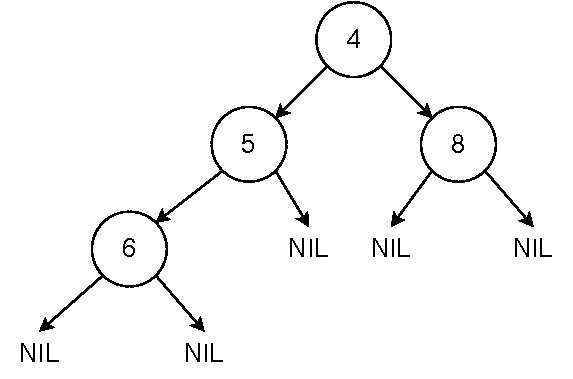
\includegraphics[scale=0.5]{img/rank}
     \caption{$rank(4) = 2$、$rank(6) = rank(8) = rank(5) = 1$} \label{fig:rank}
   \end{center}
\end{figure}

\subsubsection{左偏性质}

使用Rank,我们可以定义合并时的策略:

\begin{itemize}
\item 总是合并右侧子树。记新的右侧子树的Rank值为$r_r$;
\item 比较左右子树的Rank值,记左子树的Rank值为$r_l$,如果$r_l < r_r$,就交换左右子树。
\end{itemize}

我们称上面的合并策略为“左偏性质”。概括来说,在一棵左偏树中,到某个外部节点的最短距离总是在右侧。

左偏树总是趋向不平衡,但是它可以维护一条重要的性质,如下面的定理所述:

\begin{theorem}
若一棵左偏树$T$包含$n$个内部节点,从根节点到达最右侧的外部节点的路径上最多含有$\lfloor \log (n+1) \rfloor$个节点。
\end{theorem}

我们这里省略了此定理的证明,读者可以参考\cite{brono-book},\cite{TAOCP-bheap}来了解证明的过程。根据此定理,沿着这一路径进行操作的算法,都可以保证$O(\lg n)$的复杂度。

我们可以在二叉树定义的基础上增加一个Rank值来定义左偏树。记非空的左偏树为$(r, k, L, R)$。下面的Haskell例子程序定义了左偏树。

\lstset{language=Haskell}
\begin{lstlisting}[style=Haskell]
data LHeap a = E -- 空
             | Node Int a (LHeap a) (LHeap a) -- Rank、元素、左、右子树
\end{lstlisting}

我们定义空树的Rank为0,否则,我们通过读取新增加的变量$r$来获得Rank值。下面的$rank(H)$函数可以获取任一情况下的值。

\be
rank(H) = \left \{
  \begin{array}
  {r@{\quad:\quad}l}
  0 & H = \phi \\
  r & H = (r, k, L, R)
  \end{array}
\right.
\ee

对应的Haskell例子程序如下:

\lstset{language=Haskell}
\begin{lstlisting}[style=Haskell]
rank E = 0
rank (Node r _ _ _) = r
\end{lstlisting}

方便起见,我们以后将$rank(H)$简记为$r_H$。

% ================================================================
%                 Merge
% ================================================================
\subsection{合并}
\index{左偏堆!合并}

为了实现合并操作,我们需要显定义一个算法用以比较左右子树的Rank值,并适当地进行子树的交换。

\be
mk(k, A, B) = \left \{
  \begin{array}
  {r@{\quad:\quad}l}
  (r_A + 1, k, B, A) & r_A < r_B \\
  (r_B + 1, k, A, B) & otherwise
  \end{array}
\right.
\ee

这一函数接受三个参数,一个key和两棵子树$A$、$B$。如果$A$的Rank较小,算法就用$B$作为左子树,$A$作为右子树来构建一棵较大的树。然后它将$A$的Rank加一作为这棵新树的Rank值,即新树的Rank值为$r_A + 1$;否则,如果$B$的Rank较小,就用A作为左子树,$B$作为右子树。新树的Rank值为$r_B + 1$。

由于构造新树的时候,我们在顶部增加了一个新的key。所以Rank的值会增长1。

给定两个左偏堆$H_1$和$H_2$,记它们的key和左右子树分别为:$k_1, L_1, R_1$和$k_2, L_2, R_2$。下面的$merge(H_1, H_2)$函数定义了合并算法:

\be
merge(H_1, H_2) = \left \{
  \begin{array}
  {r@{\quad:\quad}l}
  H_2 & H_1 = \phi \\
  H_1 & H_2 = \phi \\
  mk(k_1, L_1, merge(R_1, H_2)) & k_1 < k_2 \\
  mk(k_2, L_2, merge(H_1, R_2)) & otherwise
  \end{array}
\right.
\ee

函数$merge$总是在右子树上进行递归调用,因此左偏的性质得以保持。这样就保证了算法的复杂度为$O(\lg n)$。

下面的Haskell例子代码实现了合并算法。

\lstset{language=Haskell}
\begin{lstlisting}[style=Haskell]
merge E h = h
merge h E = h
merge h1@(Node _ x l r) h2@(Node _ y l' r') =
    if x < y then makeNode x l (merge r h2)
    else makeNode y l' (merge h1 r')

makeNode x a b = if rank a < rank b then Node (rank a + 1) x b a
                 else Node (rank b + 1) x a b
\end{lstlisting}

\subsubsection{合并由数组表示的二叉堆}
\index{二叉堆!合并}

使用数组表示的二叉堆在大多数情况下速度都很快。并且很和现代计算机的高速缓存技术(cache)配合良好。但是合并操作的算法复杂度却为线性时间$O(n)$。通常的实现是将两个数组连接起来,然后在连接后的结果上重新构建堆\cite{NIST}。

\begin{algorithmic}[1]
\Function{Merge-Heap}{$A, B$}
  \State $C \gets$ \Call{Concat}{$A, B$}
  \State \Call{Build-Heap}{$C$}
\EndFunction
\end{algorithmic}

% ================================================================
%                 Basic heap operations
% ================================================================
\subsection{基本堆操作}

使用此前定义的$merge$算法,我们可以实现很多基本的堆操作。

\subsubsection{获取顶部元素和弹出操作}
\index{左偏堆!top}
\index{左偏堆!pop}
\index{左偏堆!弹出}

由于最小的元素总是存储于根节点,我们可以在常数时间$O(1)$内获取到堆的顶部元素。下式从非空的堆$H = (r, k, L, R)$中获取顶部元素。我们忽略了树为空时的错误处理。

\be
top(H) = k
\ee

为了实现弹出操作,我们首先将顶部元素删除,然后将左右子树合并为一个新的堆。

\be
pop(H) = merge(L, R)
\ee

由于弹出算法的实现直接调用了$merge$函数,因此左偏树弹出操作的复杂度也是$O(\lg n)$。

\subsubsection{插入}
\index{左偏树!插入}

我们可以从待插入的元素构建一棵只有一个叶子节点的树,然后将它和已有的左偏树合并到一起。

\be
insert(H, k) = merge(H, (1, k, \phi, \phi))
\ee

显然,由于直接调用$merge$函数,这一算法的复杂度也是$O(\lg n)$。

使用插入操作,我们可以很容易地将一个列表中的元素依次插入到左偏堆中。下面的构造算法使用了folding。

\be
build(L) = fold(insert, \phi, L)
\ee

图\ref{fig:leftist-tree}给出另一个构造左偏树的例子。

\begin{figure}[htbp]
   \begin{center}
   	  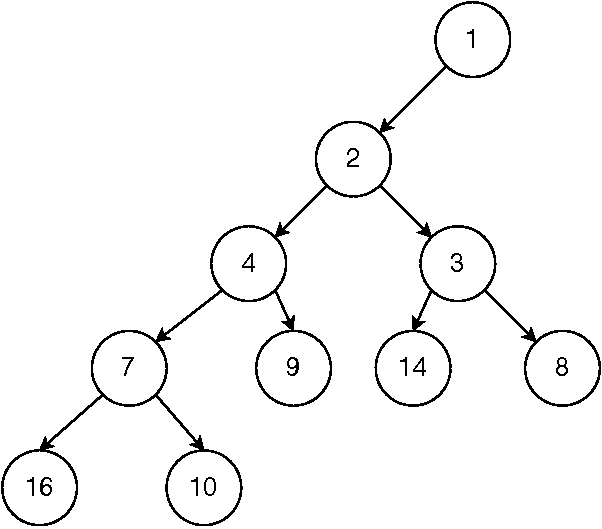
\includegraphics[scale=0.5]{img/leftist-tree}
    \caption{从列表$\{9, 4, 16, 7, 10, 2, 14, 3, 8, 1\}$构造左偏树}
    \label{fig:leftist-tree}
   \end{center}
\end{figure}

下面的Haskell例子程序实现了上面的各个左偏树操作。

\lstset{language=Haskell}
\begin{lstlisting}[style=Haskell]
insert h x = merge (Node 1 x E E) h

findMin (Node _ x _ _) = x

deleteMin (Node _ _ l r) = merge l r

fromList = foldl insert E
\end{lstlisting}

% ================================================================
%                 Heap sort
% ================================================================
\subsection{使用左偏堆实现堆排序}
\index{左偏树!堆排序}

使用堆的基本操作,我们可以给出堆排序的实现。给定一个序列,我们首先将它转换成一个左偏堆,然后不断从堆中取得最小元素。

\be
sort(L) = heapSort(build(L))
\ee

\be
heapSort(H) = \left \{
  \begin{array}
  {r@{\quad:\quad}l}
  \phi & H = \phi \\
  \{top(H)\} \cup heapSort(pop(H)) & otherwise
  \end{array}
\right.
\ee

因为弹出操作的复杂度是对数时间的,并且被调用了$n$次,因此排序的总体复杂度为$O(n \lg n)$。下面的Haskell例子程序实现了左偏树的堆排序。

\lstset{language=Haskell}
\begin{lstlisting}[style=Haskell]
heapSort = hsort . fromList where
    hsort E = []
    hsort h = (findMin h):(hsort $ deleteMin h)
\end{lstlisting} %$



% ================================================================
%                 Skew Heap
% ================================================================

\subsection{Skew堆}
\label{skew-heap}
\index{Skew堆}

左偏堆在某些情况下会产生很不平衡的结构。图\ref{fig:unbalanced-leftist-tree}给出了一个例子,依次将序列$\{16, 14, 10, 8, 7, 9, 3, 2, 4, 1\}$中的元素插入到左偏堆。

\begin{figure}[htbp]
   \begin{center}
   	  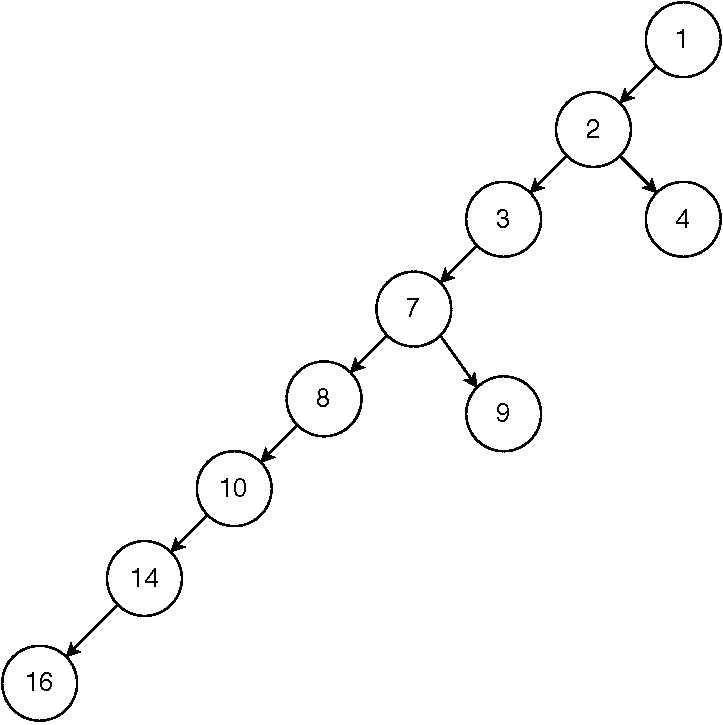
\includegraphics[scale=0.3]{img/unbalanced-leftist-tree}
    \caption{从序列$\{16, 14, 10, 8, 7, 9, 3, 2, 4, 1\}$构造的左偏堆很不平衡}
    \label{fig:unbalanced-leftist-tree}
   \end{center}
\end{figure}

Skew堆(或称\underline{自调整堆})既简化了左偏堆的实现,又提高了平衡性\cite{wiki-skew-heap}、\cite{self-adjusting-heaps}。

在构造左偏堆的时候,如果左侧的Rank值小于右侧的,我们就交换左右子树。但是这一“比较―交换”的策略在merge时不能很好处理某一分支为叶子节点的情况。这是因为,不管这棵树有多大,它的Rank值总为1。一种“简单粗暴”的解决方式是,每次合并,我们都交换左右子树。这就是Skew堆的原理。

\subsubsection{Skew堆的定义}

Skew堆是由skew树实现的堆。Skew树是一种特殊的二叉树。最小的元素保存在根节点,每棵子树也都是一棵skew树。

Skew树无需保存Rank值(或$S$值)。我们可以直接复用二叉树的定义。树或者为空,或者记为前序形式$(k, L, R)$。下面的Haskell例子代码定义了skew树。

\lstset{language=Haskell}
\begin{lstlisting}[style=Haskell]
data SHeap a = E -- 空
             | Node a (SHeap a) (SHeap a) -- 元素、左、右
\end{lstlisting}

\subsubsection{合并}
\index{Skew堆!合并}
\index{Skew堆!插入}
\index{Skew堆!top}
\index{Skew堆!pop}
\index{Skew堆!弹出}

合并算法被大幅度简化:当合并两棵非空skew树时,我们比较根节点,选择较小的作为新的根。然后把含有较大元素的树合并到某一子树上。最后再把左右子树交换。记两棵非空子树为:$H_1 = (k_1, L_1, R_1)$和$H_2 =(k_2, L_2, R_2)$。若$k_1 < k_2$,选择$k_1$作为新的根。我们既可以将$H_2$和$L_1$合并,也可以将$H_2$和$R_1$合并。不失一般性,我们合并到$R_1$上。然后交换左右子树,最后的结果为$(k_1, merge(R_1, H_2), L_1)$。考虑边界情况,最终的算法定义如下:

\be
merge(H_1, H_2) = \left \{
  \begin{array}
  {r@{\quad:\quad}l}
  H_1 & H_2 = \phi \\
  H_2 & H_1 = \phi \\
  (k_1, merge(R_1, H_2), L_1) & k_1 < k_2 \\
  (k_2, merge(H_1, R_2), L_2) & otherwise
  \end{array}
\right.
\ee

其他的操作,包括插入,获取顶部元素和弹出都和左偏树一样通过调用merge来实现。唯一的不同是我们不再需要Rank了。

下面的Haskell例子程序实现了skew堆。

\lstset{language=Haskell}
\begin{lstlisting}element, left, right
merge E h = h
merge h E = h
merge h1@(Node x l r) h2@(Node y l' r') =
    if x < y then Node x (merge r h2) l
    else Node y (merge h1 r') l'

insert h x = merge (Node x E E) h

findMin (Node x _ _) = x

deleteMin (Node _ l r) = merge l r
\end{lstlisting}

即使我们用skew堆处理已序序列,结果仍然是一棵较平衡的二叉树,如图\ref{fig:skew-tree}所示。

\begin{figure}[htbp]
   \begin{center}
   	  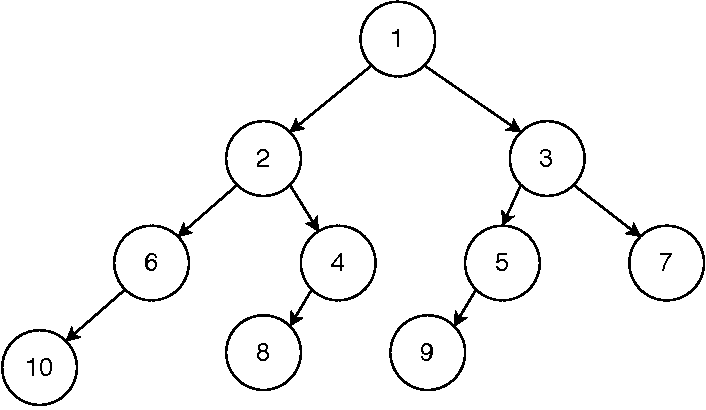
\includegraphics[scale=0.5]{img/skew-tree}
    \caption{用已序序列$\{1, 2, ..., 10\}$构造的skew树仍然比较平衡}
    \label{fig:skew-tree}
   \end{center}
\end{figure}


% ================================================================
%                 Splay Heap
% ================================================================

\section{伸展堆}
\label{splayheap}
\index{伸展堆}

左偏堆和skew堆说明,使用二叉树完全可以实现堆这种数据结构。而且skew堆还给出了一种解决树平衡的方法。本节介绍的伸展堆给出了另外一种改善平衡性的方法。

左偏堆和skew堆使用的树都不是二叉搜索树(BST)。如果我们将底层的数据结构换成二叉搜索树,最小(或最大)元素就不再保存于根节点。我们需要$O(\lg n)$时间来获取最小(或最大)元素。

如果二叉搜索树不平衡,性能会大幅下降。最坏情况下,大部分操作都退化为$O(n)$。虽然我们可以用红黑树来实现二叉堆,但这太复杂了。伸展树提供了一种轻量级的实现,它的结果可以动态趋向平衡。


% ================================================================
%                 Definition
% ================================================================
\subsection{定义}

伸展树采用类似于缓存(cache)的策略,它不断将当前正在访问的节点向top旋转,这样再次访问的时候就可以更快。我们将这样的操作称为“伸展(splay)”。对于不平衡的二叉搜索树,经过若干次伸展操作后,树会变得越来越平衡。大多数伸展树操作的均摊(amortized)性能都是$O(\lg n)$的。Daniel Dominic Sleator和Robert Endre Tarjan在1985年最早引入了伸展树\cite{wiki-splay-tree}\cite{self-adjusting-trees}。

\subsubsection{伸展操作}
\index{伸展堆!splaying}

有两种方法可以实现伸展操作。第一种需要处理较多的情况,但可以很容易地使用模式匹配(pattern matching)来实现;第二种具备统一的形式,但是实现较为复杂。

记当前正在访问的节点为$X$,它的父节点为$P$,如果存在祖父节点,则记为$G$。伸展操作分为三各步骤,每个步骤有两个对称的情况,为了节省篇幅,我们只给出每步中的一种情况。

\begin{itemize}
\item \underline{Zig-zig}步骤,如图\ref{fig:zig-zig}所示,$X$和$P$都是左子树或者$X$和$P$都是右子树。我们通过两次旋转,将$X$变成根节点。

\begin{figure}[htbp]
  \centering
  \subcaptionbox{$X$和$P$都是左子树或者$X$和$P$都是右子树。}{\includegraphics[scale=0.4]{img/zig-zig-a}}
  \subcaptionbox{$X$经过两次旋转后成为了根节点。}{\includegraphics[scale=0.4]{img/zig-zig-b}}
  \caption{Zig-zig情况} \label{fig:zig-zig}
\end{figure}

\item \underline{Zig-zag}步骤,如图\ref{fig:zig-zag}所示,$X$和$P$一棵是左子树另一棵是右子树。经过旋转,$X$变成根节点,$P$和$G$变成了兄弟节点。

\begin{figure}[htbp]
  \centering
  \subcaptionbox{$X$和$P$一棵是左子树另一棵是右子树。}{\includegraphics[scale=0.4]{img/zig-zag-a}}
  \subcaptionbox{$X$成为根节点,$P$和$G$变成了兄弟节点。}{\includegraphics[scale=0.4]{img/zig-zag-b}}
  \caption{Zig-zag情况} \label{fig:zig-zag}
\end{figure}

\item \underline{Zig}步骤,如图\ref{fig:zig}所示,这种情况下,$P$是根节点,经过旋转,$X$变成了根节点。这是伸展操作的最后一步。

\begin{figure}[htbp]
  \centering
  \subcaptionbox{$P$是根节点。}{\includegraphics[scale=0.4]{img/zig-a}}
  \subcaptionbox{通过旋转将$X$变为根节点。}{\includegraphics[scale=0.4]{img/zig-b}}
  \caption{Zig情况} \label{fig:zig}
\end{figure}

\end{itemize}

虽然有6种不同的情况,但是它们可以很容易地用模式匹配来处理。记非空二叉树为$T=(L, k, R)$,当访问树中的节点$Y$时,伸展操作可以定义如下:

\be
splay(T, X) = \left \{
  \begin{array}
  {r@{\quad:\quad}l}
  (a, X, (b, P, (c, G, d))) & T = (((a, X, b), P, c), G, d), X = Y \\
  (((a, G, b), P, c), X, d) & T= (a, G, (b, P, (c, X, d))), X = Y \\
  ((a, P, b), X, (c, G, d)) & T = (a, P, (b, X, c), G, d), X = Y \\
  ((a, G, b), X, (c, P, d)) & T = (a, G, ((b, X, c), P, d)), X = Y \\
  (a, X, (b, P, c)) & T = ((a, X, b), P, c), X = Y \\
  ((a, P, b), X, c) & T = (a, P, (b, X, c)), X = Y \\
  T &  otherwise
  \end{array}
\right.
\ee

前两条子式处理“zig-zig”情况;接下来的两条子式处理“zig-zag”情况;最后两条子式处理“zig”情况。其他情况下,树都保持不变。

下面的Haskell例子程序实现了伸展操作。

\lstset{language=Haskell}
\begin{lstlisting}[style=Haskell]
data STree a = E -- 空
             | Node (STree a) a (STree a) -- left, key, right

-- zig-zig
splay t@(Node (Node (Node a x b) p c) g d) y =
    if x == y then Node a x (Node b p (Node c g d)) else t
splay t@(Node a g (Node b p (Node c x d))) y =
    if x == y then Node (Node (Node a g b) p c) x d else t
-- zig-zag
splay t@(Node (Node a p (Node b x c)) g d) y =
    if x == y then Node (Node a p b) x (Node c g d) else t
splay t@(Node a g (Node (Node b x c) p d)) y =
    if x == y then Node (Node a g b) x (Node c p d) else t
-- zig
splay t@(Node (Node a x b) p c) y = if x == y then Node a x (Node b p c) else t
splay t@(Node a p (Node b x c)) y = if x == y then Node (Node a p b) x c else t
-- 否则
splay t _ = t
\end{lstlisting}

每次插入新key时,我们就执行伸展操作来调整树的平衡性。如果树为空,结果为一个叶子节点;否则我们比较待插入的key和根节点,如果待插入的key较小,就将其递归插入左子树,然后执行伸展操作;否则将key插入右子树,再执行伸展操作。

\be
insert(T, x) = \left \{
  \begin{array}
  {r@{\quad:\quad}l}
  (\phi, x, \phi) & T = \phi \\
  splay((insert(L, x), k, R), x) & T = (L, k, R), x < k \\
  splay(L, k, insert(R, x)) & otherwise
  \end{array}
  \right.
\ee

下面的Haskell程序实现了插入算法。

\lstset{language=Haskell}
\begin{lstlisting}[style=Haskell]
insert E y = Node E y E
insert (Node l x r) y
    | x > y     = splay (Node (insert l y) x r) y
    | otherwise = splay (Node l x (insert r y)) y
\end{lstlisting}

图\ref{fig:splay-result}描述了向伸展树插入逐一插入有序序列$\{1, 2, ..., 10\}$中元素的结果。如果使用普通二叉树,会退化成一条链表。而伸展树则产生比较平衡的结果。

\begin{figure}[htbp]
  \centering
  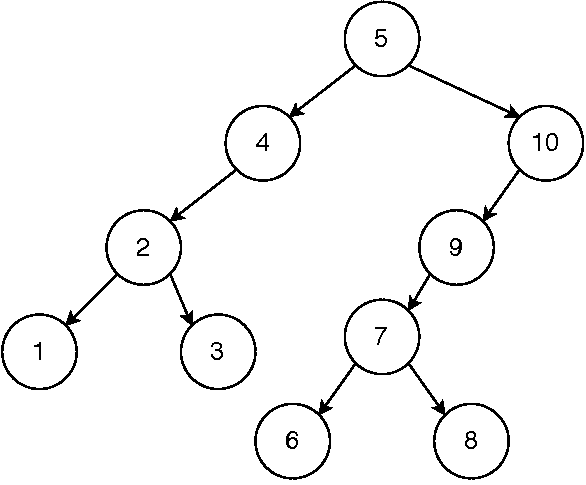
\includegraphics[scale=0.5]{img/splay-tree}
  \caption{伸展操作可以改善平衡性}
  \label{fig:splay-result}
\end{figure}

Okasaki发现了一条简单的伸展操作规则\cite{okasaki-book}:每次连续向左或者向右访问两次的时候,就旋转两个节点。

根据这一规则,我们可以这样实现伸展:当访问节点$x$的时候(插入、查找或者删除时),如果连续向左侧或者右侧前进两次,我们就将树分割成两部分:$L$和$R$,其中$L$含有所有小于$x$的节点,$R$含有其余的节点。我们可以构建一棵新树(例如插入时),将$x$作为根,$L$和$R$分别作为左右子树。分割是递归的,它会对子树也进行伸展操作。

\be
partition(T, p) = \left \{
  \begin{array}
  {r@{\quad:\quad}l}
  (\phi, \phi) & T = \phi \\
  (T, \phi) & T = (L, k, R) \land R = \phi \\
  ((L, k, L'), k', A, B) & \begin{array}{l} \\
                             T = (L, k, (L', k', R')) \\
                             k < p, k' < p \\
                             (A, B) = partition(R', p)
                           \end{array} \\
  ((L, k, A), (B, k', R')) & \begin{array}{l} \\
                               T = (L, K, (L', k', R')) \\
                               k < p \leq k' \\
                               (A, B) = partition(L', p) \\ \\
                             \end{array} \\
  (\phi, T) & T = (L, k, R) \land L = \phi \\
  (A, (L', k', (R', k, R)) & \begin{array}{l} \\
                               T = ((L', k', R'), k, R) \\
                               p \leq k, p \leq k' \\
                               (A, B) = partition(L', p)
                             \end{array} \\
  ((L', k', A), (B, k, R)) & \begin{array}{l} \\
                               T = ((L', k', R'), k, R) \\
                               k' \leq p \leq k \\
                               (A, B) = partition(R', p)
                             \end{array}
  \end{array}
  \right.
\ee

函数$partition(T, p)$接受一棵树$T$和一个基准值(pivot)$p$为参数。第一条子式处理边界条件。对空树进行分割的结果为一对空的左右子树。否则,记树为$(L, k, R)$,我们需要比较基准值$p$和根节点的值$k$。如果$k < p$,分为两种子情况。一种是$R$为空的简单情况,根据二叉搜索树的性质,所有的元素都小于$p$,因此结果为$(T, \phi)$。

否则,$R = (L', k', R')$,我们需要递归地用基准值分割$R'$,将$R'$中所有小于$p$的元素放入树$A$,其余元素放入树$B$。结果为一对树,其中一棵为$((L, k, L'), k', A)$,另一棵为$B$。

如果右子树的key不小于基准值,我们递归地用基准值分割$L'$得到结果$(A, B)$。最终的结果为一对树,一棵是$(L, k, A)$,另一棵是$(B, k', R')$。当$p \leq k$时,情况是对称的,由最后的三条子式处理。

下面的Haskell例子程序实现了分割算法。

\begin{lstlisting}[style=Haskell]
partition E _ = (E, E)
partition t@(Node l x r) y
    | x < y =
        case r of
          E -> (t, E)
          Node l' x' r' ->
              if x' < y then
                  let (small, big) = partition r' y in
                  (Node (Node l x l') x' small, big)
              else
                  let (small, big) = partition l' y in
                  (Node l x small, Node big x' r')
    | otherwise =
        case l of
          E -> (E, t)
          Node l' x' r' ->
              if y < x' then
                  let (small, big) = partition l' y in
                  (small, Node l' x' (Node r' x r))
              else
                  let (small, big) = partition r' y in
                  (Node l' x' small, Node big x r)
\end{lstlisting}

% ================================================================
%                 Basic heap operations
% ================================================================
\index{伸展堆!插入}
我们可以用$partition$实现插入算法。当向一个伸展堆$T$插入一个新元素$k$时,我们先将堆分割为两棵子树$L$和$R$。其中$L$含有所有小于$k$的节点,而$R$含有剩余的部分。然后我们构建一棵新树,使用$k$作为根,$L$和$R$作为子树。

\be
insert(T, k) = (L, k, R), (L, R) = partition(T, k)
\ee

对应的Haskell例子程序如下:

\lstset{language=Haskell}
\begin{lstlisting}[style=Haskell]
insert t x = Node small x big where (small, big) = partition t x
\end{lstlisting}

\subsubsection{获取和弹出顶部元素}
\index{伸展堆!top}
\index{伸展堆!pop}
\index{伸展堆!弹出}

由于伸展树本质上是二叉搜索树,最小的元素存储于最左侧的节点中。我们需要不断向左遍历以获取顶部元素。记非空的树为$T=(L, k, R)$,$top(T)$函数可以定义如下:

\be
top(T) = \left \{
  \begin{array}
  {r@{\quad:\quad}l}
  k & L = \phi \\
  top(L) & otherwise
  \end{array}
  \right.
\ee

这实际上就是二叉搜索树的$min(T)$算法。

对于弹出操作,算法需要将最小元素删除。每当连续向左访问两次,就执行一次伸展操作。

\be
pop(T) = \left \{
  \begin{array}
  {r@{\quad:\quad}l}
  R & T = (\phi, k, R) \\
  (R', k, R) & T = ((\phi, k', R'), k, R) \\
  (pop(L'), k', (R', k, R)) & T = ((L', k', R'), k, R)
  \end{array}
  \right.
\ee

注意这里的第三条子式实际上执行了伸展操作,它并没有显式地调用$partition$函数,而是直接使用了二叉搜索树的性质。

因为伸展树是平衡的,top和pop操作的性能都是$O(\lg n)$。

下面的Haskell例子程序实现了top和pop操作。

\lstset{language=Haskell}
\begin{lstlisting}[style=Haskell]
findMin (Node E x _) = x
findMin (Node l x _) = findMin l

deleteMin (Node E x r) = r
deleteMin (Node (Node E x' r') x r) = Node r' x r
deleteMin (Node (Node l' x' r') x r) = Node (deleteMin l') x' (Node r' x r)
\end{lstlisting}

\subsubsection{合并}
\index{伸展堆!合并}

合并是堆的一个重要操作,它被广泛用于图算法。通过使用$partition$函数,我们可以实现一个$O(\lg n)$时间的合并算法。

当合并两棵伸展树时,如果它们都不为空,我们可以将第一棵树的根节点作为新的根,然后将其作为基准值分割第二棵树。此后,我们递归地将第一棵树的子树合并。算法定义如下:

\be
merge(T_1, T_2) = \left \{
  \begin{array}
  {r@{\quad:\quad}l}
  T_2 & T_1 = \phi \\
  (merge(L, A), k, merge(R, B)) & T_1 = (L, k, R), (A, B) = partition(T_2, k)
  \end{array}
  \right.
\ee

如果第一个堆为空,结果显然为第二个堆。否则,记第一个堆为$(L, k, R)$,我们使用$k$作为基准值分割$T_2$得到结果$(A, B)$,其中$A$包含$T_2$中所有小于$k$的节点,而$B$包含其余节点。我们接下来递归地将$A$和$L$合并为新的左子树,将$B$和$R$合并为右子树。

这一定义可以翻译为下面的Haskell例子程序。

\lstset{language=Haskell}
\begin{lstlisting}[style=Haskell]
merge E t = t
merge (Node l x r) t = Node (merge l l') x (merge r r')
    where (l', r') = partition t x
\end{lstlisting}

% ================================================================
%                 Heap sort
% ================================================================
\subsection{堆排序}

由于伸展堆的内部实现对于通用堆的接口完全透明,我们可以完全复用此前的堆排序定义。也就是说堆排序的算法也是通用的,它不依赖于底层的数据结构。

% ================================================================
%                 Short summary
% ================================================================
\section{小结}

本章中,我们介绍了通用的二叉堆概念。只要保证堆的性质,我们可以使用任何形式的二叉树来实现堆。

这样的定义并不仅限于使用基于数组的二叉堆,它也包含使用其他二叉树形式的堆如左偏堆、skew堆和伸展堆。基于数组的二叉堆易于用命令式的方式实现。它将一棵完全二叉树映射为数组的随机访问,我们很难找到和它直接对应的纯函数式实现。

但是,我们可以通过使用显式的二叉树来实现纯函数式的二叉堆。大部分的操作在最坏情况下也可以达到$O(\lg n)$的性能。有些操作的分摊性能甚至可以达到$O(1)$。Okasaki在\cite{okasaki-book}中给出了这些数据结构的详细分析。

我们仅在本章中给出了左偏堆、skew堆和伸展堆的纯函数式实现。它们也都支持命令式实现。

人们很自然希望能将二叉树扩展到$k$叉树,这样就会得到其他重要的数据结构如二项式(Binomial)堆、斐波那契(Fibonacci)堆和配对(pairing)堆。我们将在后面的章节加以介绍。

% ================================================================
%                 Exercise
% ================================================================
\begin{Exercise}
\begin{itemize}
\item 用命令式的方式实现左偏堆、skew堆和伸展堆。
\end{itemize}
\end{Exercise}

\ifx\wholebook\relax \else
\begin{thebibliography}{99}

\bibitem{CLRS}
Thomas H. Cormen, Charles E. Leiserson, Ronald L. Rivest and Clifford Stein. ``Introduction to Algorithms, Second Edition''. The MIT Press, 2001. ISBN: 0262032937.(《算法导论》)

\bibitem{wiki-heap}
Heap (data structure), Wikipedia. \url{https://en.wikipedia.org/wiki/Heap_(data_structure)}

\bibitem{wiki-heapsort}
Heapsort, Wikipedia. \url{https://en.wikipedia.org/wiki/Heapsort}

\bibitem{okasaki-book}
Chris Okasaki. ``Purely Functional Data Structures''. Cambridge university press, (July 1, 1999), ISBN-13: 978-0521663502

\bibitem{rosetta-heapsort}
Sorting algorithms/Heapsort. Rosetta Code. \url{http://rosettacode.org/wiki/Sorting_algorithms/Heapsort}

\bibitem{wiki-leftist-tree}
Leftist Tree, Wikipedia. \url{https://en.wikipedia.org/wiki/Leftist_tree}

\bibitem{brono-book}
Bruno R. Preiss. Data Structures and Algorithms with Object-Oriented Design Patterns in Java. \url{http://www.brpreiss.com/books/opus5/index.html}

\bibitem{TAOCP-bheap}
Donald E. Knuth. ``The Art of Computer Programming. Volume 3: Sorting and Searching.''. Addison-Wesley Professional;
2nd Edition (October 15, 1998). ISBN-13: 978-0201485417. Section 5.2.3 and 6.2.3

\bibitem{wiki-skew-heap}
Skew heap, Wikipedia. \url{https://en.wikipedia.org/wiki/Skew_heap}

\bibitem{self-adjusting-heaps}
Sleator, Daniel Dominic; Jarjan, Robert Endre. ``Self-adjusting heaps'' SIAM Journal on Computing 15(1):52-69. doi:10.1137/0215004 ISSN 00975397 (1986)

\bibitem{wiki-splay-tree}
Splay tree, Wikipedia. \url{https://en.wikipedia.org/wiki/Splay_tree}

\bibitem{self-adjusting-trees}
Sleator, Daniel D.; Tarjan, Robert E. (1985), ``Self-Adjusting Binary Search Trees'', Journal of the ACM 32(3):652 - 686, doi: 10.1145/3828.3835

\bibitem{NIST}
NIST, ``binary heap''. \url{http://xw2k.nist.gov/dads//HTML/binaryheap.html}

\end{thebibliography}

\end{document}
\fi
